\newcommand{\upcite}[1]{\textsuperscript{\textsuperscript{\cite{#1}}}}
\chapter{概论}
\section{交互式神经元重建系统的背景与意义}

原始神经元图像信息的神经元追踪和数字重建是神经科学界热门方向。神经元的形态反应出它的功能,相同功能的神经元通常具有类似的功能。神经科学家通过结构脑图谱的重建,可以反推大脑是如何运作,对理解智慧的产生有重要的帮助。十九世纪以来,神经科学家们开始推测记忆,甚至个性与智力都储存大脑神经元之间的连接里。图 \ref{worm} 展示了秀丽隐杆线虫的神经结构的神经结构,图中每一个节点均代表一个神经元,每一条线代表一个连接。它仅仅由 300 个神经元组成,之间的连接也仅有 7000 个。

\begin{figure}
\centering
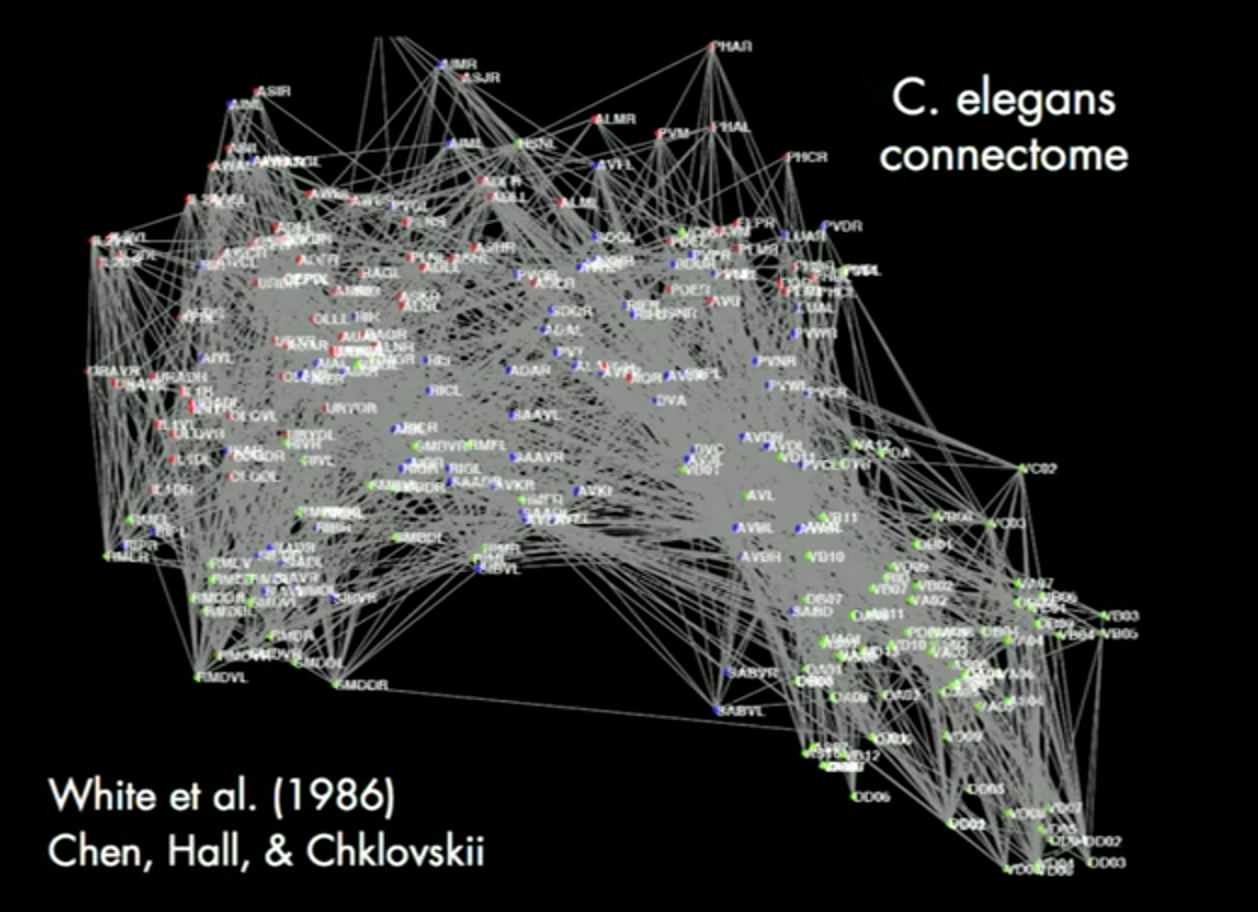
\includegraphics[width=108mm]{images/worm}
\caption{秀丽隐杆线虫的神经结构}
\label{worm}
\end{figure}

White, John G 与 Southgate 等人在 1986 年时已经 利用一系列局部原始电子显微照片对秀丽隐杆线虫的神经系统的进行了完整重建\upcite{white1986structure}。经过了 30 多年的发展,Yunkyu Sohn,Myung-Kyu Choi 与 Yong-Yeol Ahn 等人于 2011 年利用基于模块化的群态检测算法发现秀丽隐杆线虫中有 5 个解剖簇及其对应的实验可识别功能电路,进一步揭示了生物电路如何产生更高阶的复杂行为\upcite{varshney2011structural}。即使如此,由于神经网络复杂的拓扑结构,神经科学家们仍旧未能充分探索通过突触交织的神经网络结构。而人类大脑由一千亿个神经元组成,神经元之间的连接的数量又是神经元数量的一万倍,比秀丽隐杆线虫的神经结构要复杂的多。设计并实现出自动神经元重建算法便成了探索神经结构的重要步骤之一。

Druckmann, Shaul 与 Feng 等人开发的神经元重建算法提供了准确的中线,直径,表面,体积和分支点位置,支持沿着神经元表面分析标记过的分子分布,还可以直接导出到建模软件。图 \ref{Druckmann} 展示了这种神经元重建算法的样例结果。Brown, Kerry M 与 Barrionuevo 等人收集了来自不同动物,脑区,神经元类型和可视化方法的六个数据集,为自动化软件所需的测试提供了基准,提高了重建的质量,同时最大限度地减少了人工的参与,极大的促进了神经元重建领域的发展\upcite{brown2011diadem}。

\begin{figure}
\centering
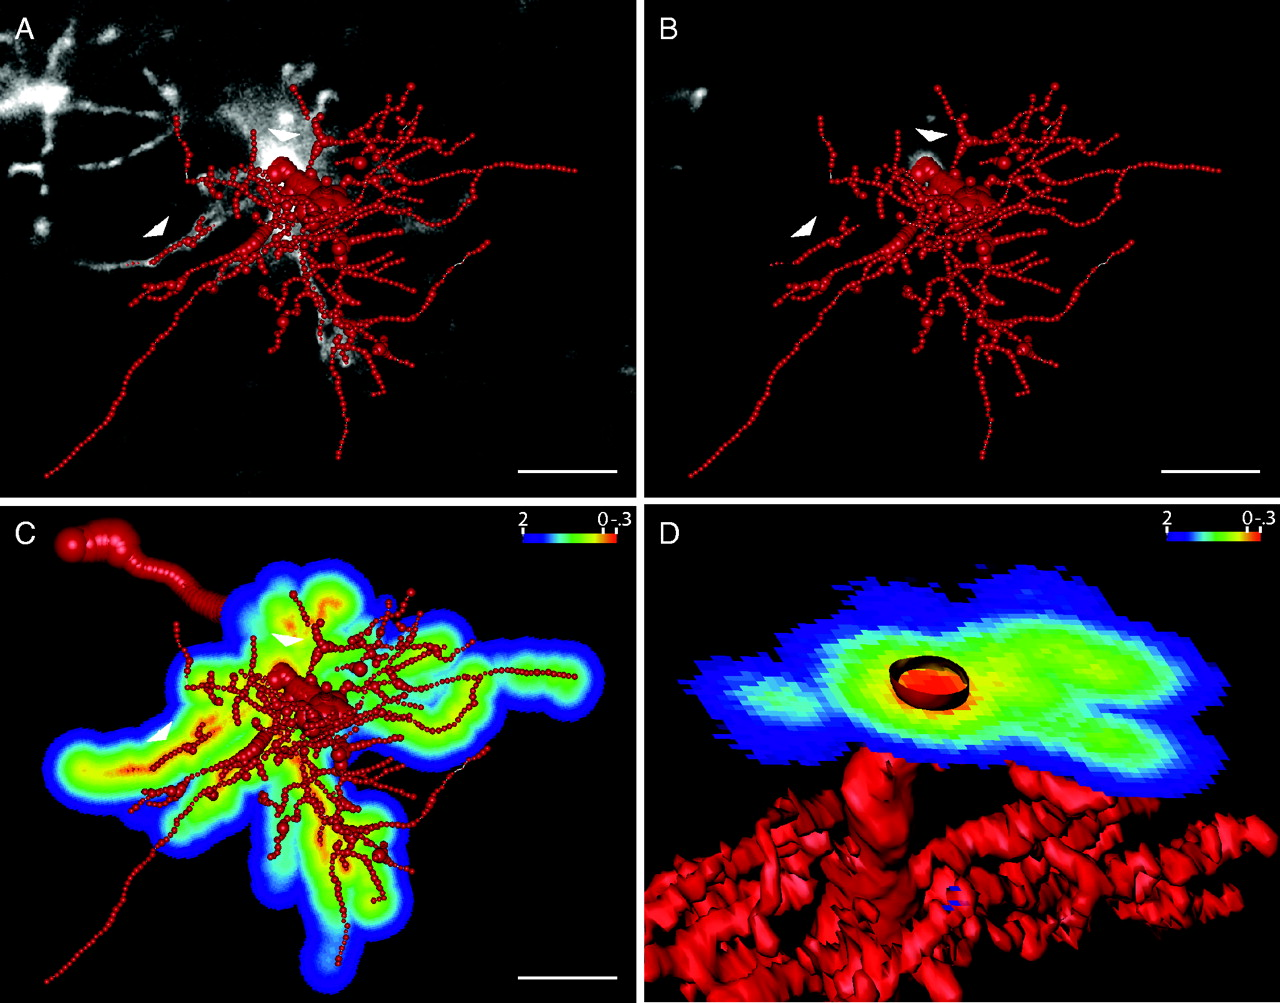
\includegraphics[width=108mm]{images/Druckmann}
\caption{Druckmann 等人的神经元重建算法的样例结果}
\label{Druckmann}
\end{figure}

由于神经元拓扑结构的复杂性,在一些自动化重建结果的细节上仍然需要研究人员对数字重建的结果进行人工纠正和修改,以确保数字重建工作的准确性。另外研究人员需要对数字重建结果进行编辑,比如添加或删除一些网络分支等。为了便于研究人员进一步研究神经结构,探索智能产生的原因,这就需要在神经元自动重建算法的基础上建立交互式神经元重建系统。

\section{现有交互式神经元重建系统的特点与问题}
\subsection{FARSIGHT}
FARSIGHT 的软件界面如图 \ref{FARSIGHT} 所示,图中正在编辑的是一小段神经结构,展示了用户点击位置,根节点方向,以及分支节点。
\begin{figure}
\centering
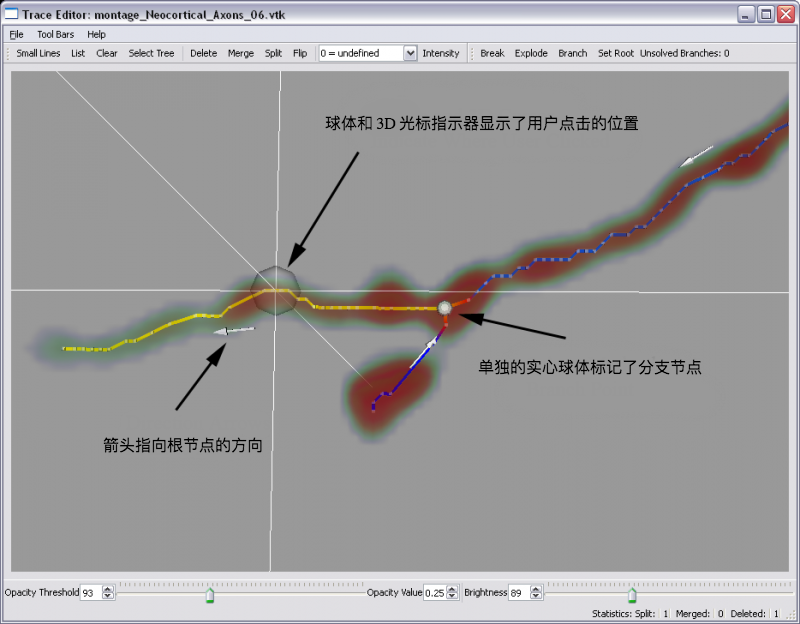
\includegraphics[width=108mm]{images/FARSIGHT}
\caption{FARSIGHT 软件运行界面}
\label{FARSIGHT}
\end{figure}

FARSIGHT 的设计目标是重建结果细节丰富,可以快速识别重建结果的错误并能迅速纠正。FARSIGHT 利用基于模式分析辅助集群编辑(PACE)的思想,根据对自动跟踪结果的定量测量和多变量模式分析工具的分析结果,发现了常见类型的重建错误,提高了纠正重建结果的效率\upcite{luisi2011farsight}。图 \ref{FARSIGHT-res} 展示了 FARSIGHT 导出的较大规模的神经结构重建结果。

\begin{figure}
\centering
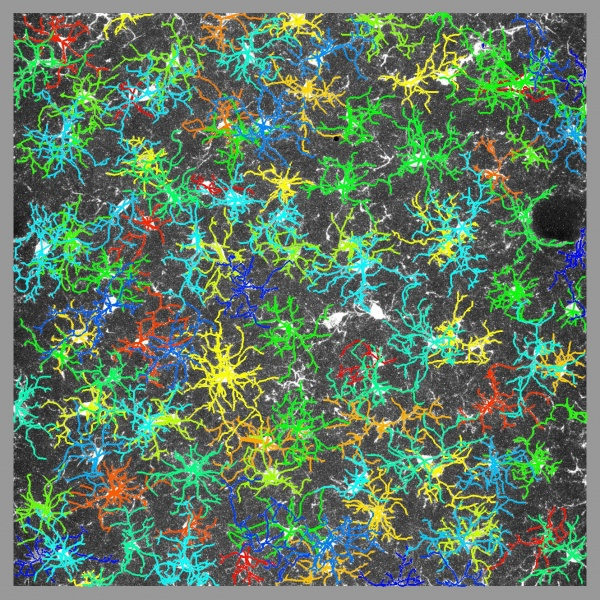
\includegraphics[width=108mm]{images/FARSIGHT-res}
\caption{FARSIGHT 导出的重建结果}
\label{FARSIGHT-res}
\end{figure}

FARSIGHT 的缺点在于,它专注于半自动重建,对于常见的错误修改效率确实较高,但是如果遇到细小的非常见错误,FARSIGHT 无法识别,也不提供精细化的编辑手段,需要借助于其他软件完成。

\subsection{neuTube}
neuTube 是一种基于 SWC 文件格式的神经元重建软件,同时具备 2D 和 3D 的可视化以及直观地编辑、绘制功能,运行用户有效的根据荧光图像数据重建神经结构,并且编辑由其他软件生成的标准神经结构的文件。软件界面如图 \ref{neutube} 所示。

\begin{figure}
\centering
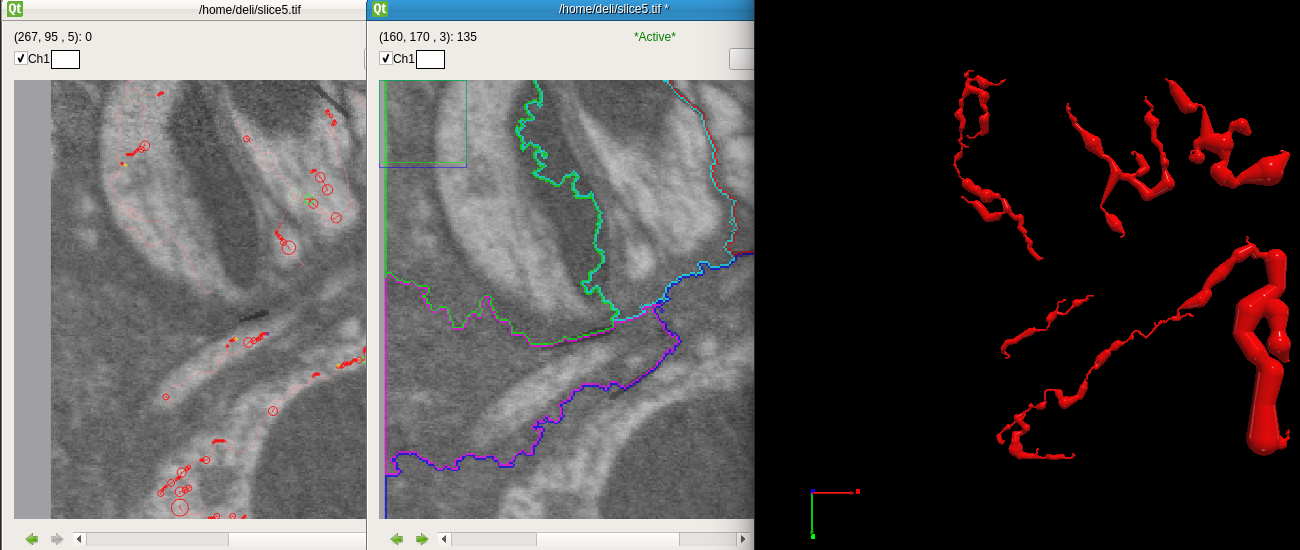
\includegraphics[width=108mm]{images/neutube}
\caption{neuTube 软件运行界面}
\label{neutube}
\end{figure}

虽然 neuTube 提供了 2D 和 3D 模式下精细编辑神经结构的功能,但是无法多人协同编辑,也无法保存编辑的历史记录,不利于多人协同工作。

\section{论文结构}
本文旨在设计并实现在线多用户的神经元网络结构编辑分享平台,利用互联网便于数据共享与交流的特点解决一些现有神经元编辑软件的问题,使得神经科学家可以便捷地进行异地,多用户协同编辑神经元网络结构,并能分享完成重建的结构脑图谱,探索神经元结构下的奥秘。由于项目涉及到数据可视化与后台服务器搭建,自然地将整个项目分成两部分,这里主要实现后台服务器的搭建,为前端可视化操作提供了有力的支持。

第一章讨论了交互式神经元重建系统的背景与意义以及神经元编辑软件的问题,第二章讨论了项目整体架构并简单介绍所用到的技术
。第三章讨论技术实现的细节以及如何根据性能测试报告进行性能优化,第四章描述了在性能优化之后的系统整体性能,第四章讨论了接下来的工作以及分析了项目中存在的不足。

